We generated datasets from the LDA model for a range of parameters,
and tested the algorithms discussed in previous section on the
prediction task. For the LDA algorithm and our Projector algorithm, we
also have results for the recovery task. We experimented with $k$ from
$3$ to $30$, and in each case, a set of $\alpha$ and $\beta$ to cover
a wide range of $sig\_word$ and $sig\_topic$. See
figure~\ref{fig:predictResult} for the prediction results of the
algorithms on a representative set of datasets.
\begin{figure}
     \begin{center}

        \subfigure{
           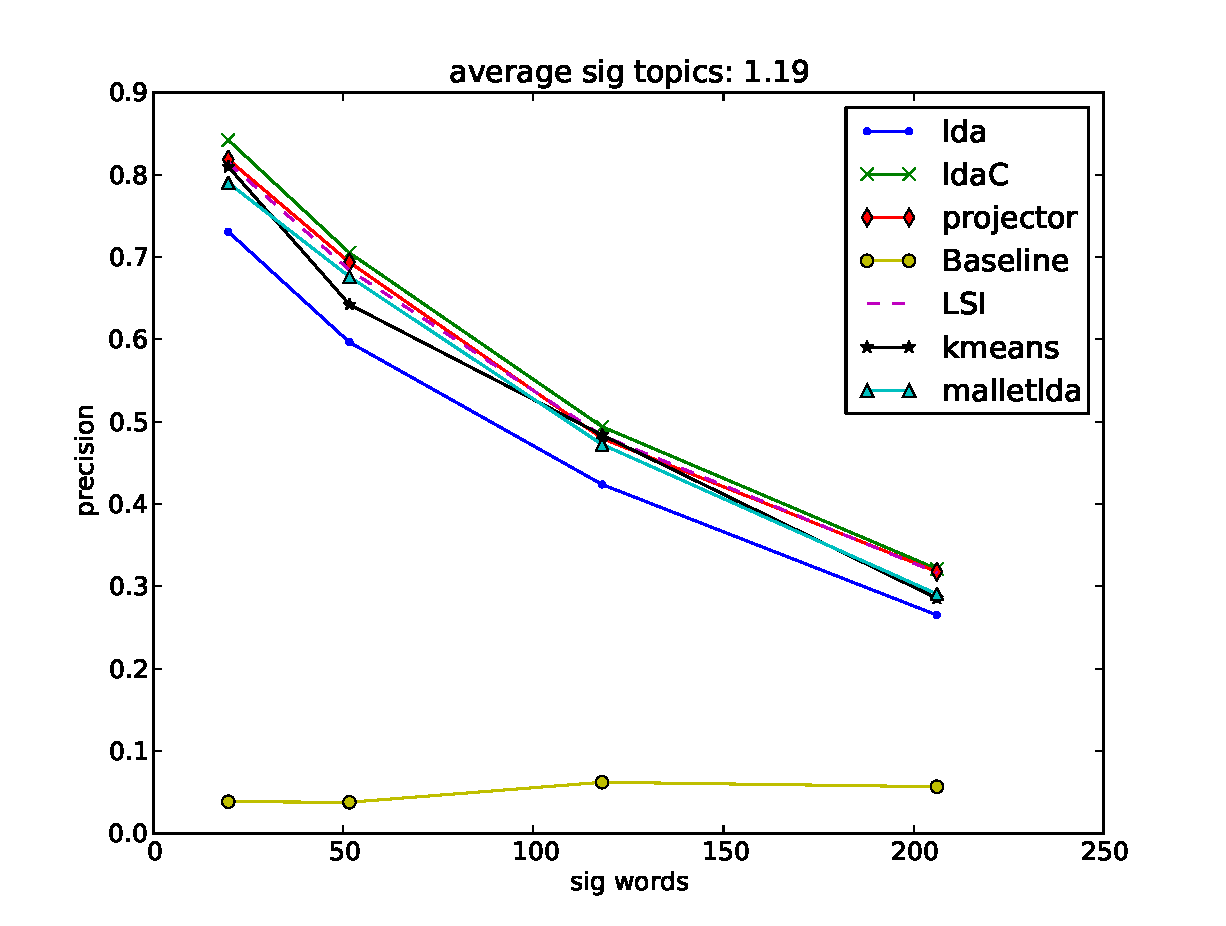
\includegraphics[width=0.4\textwidth]{k15a1.pdf}      
            %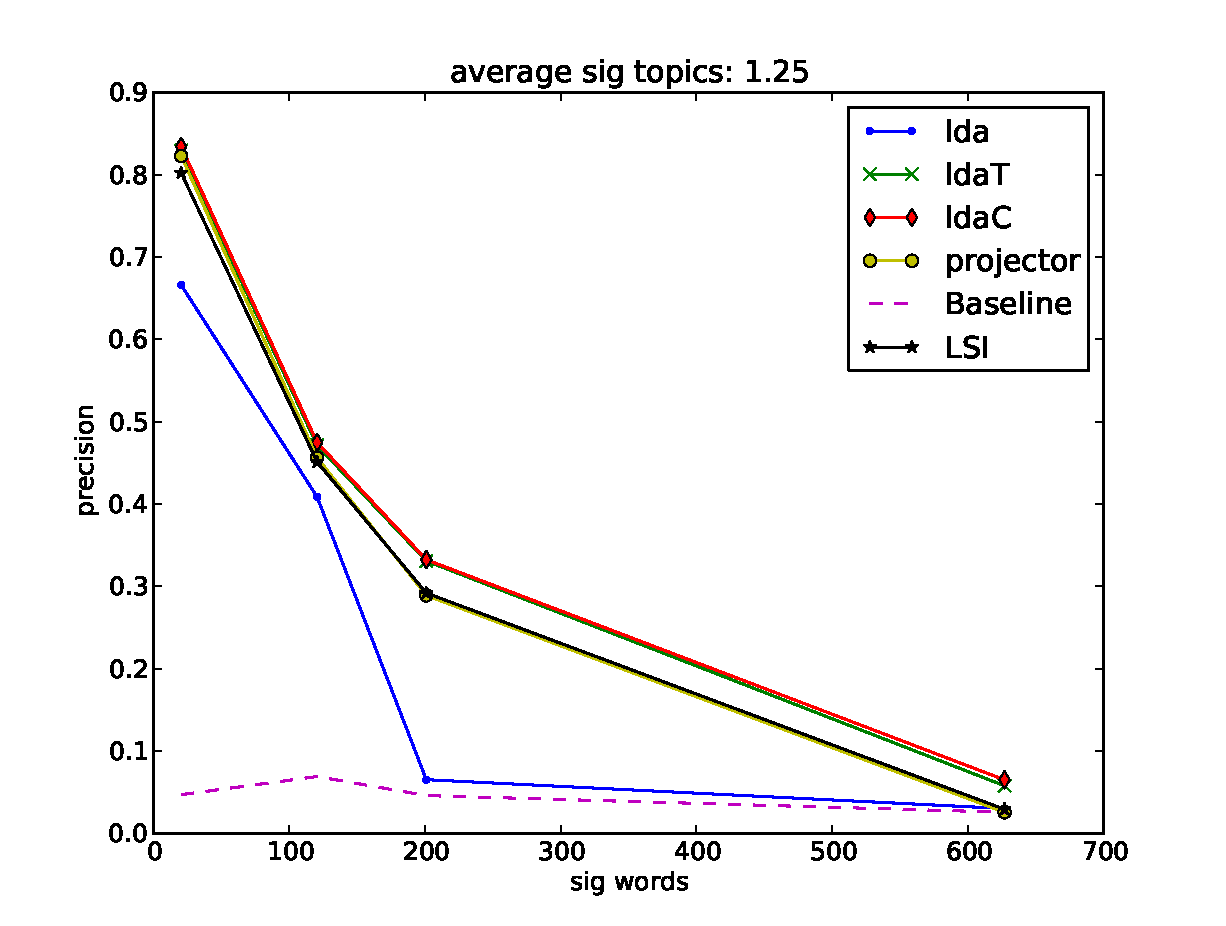
\includegraphics[width=0.4\textwidth]{k20a125.pdf}
        }
        \subfigure{
           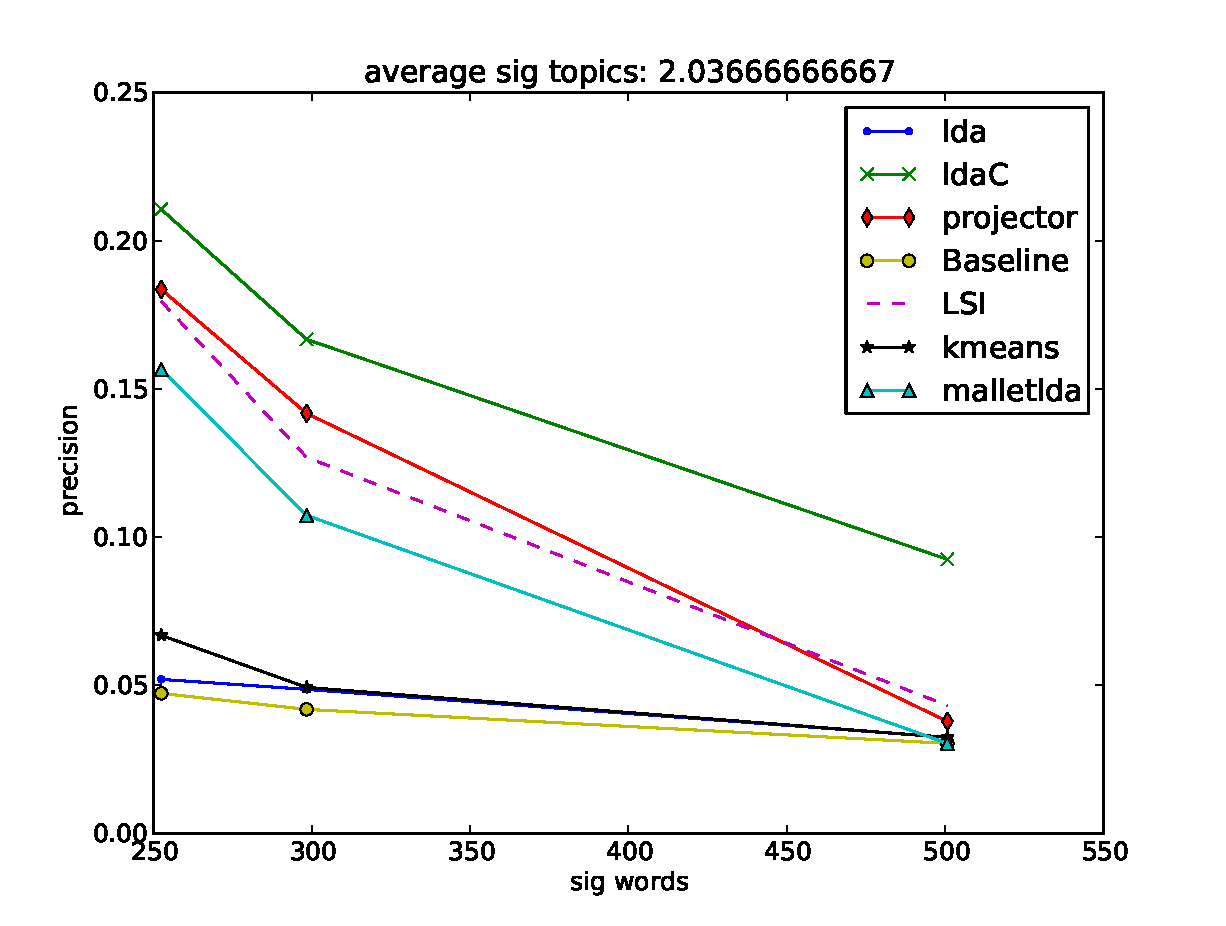
\includegraphics[width=0.4\textwidth]{k15a2.pdf}      
           %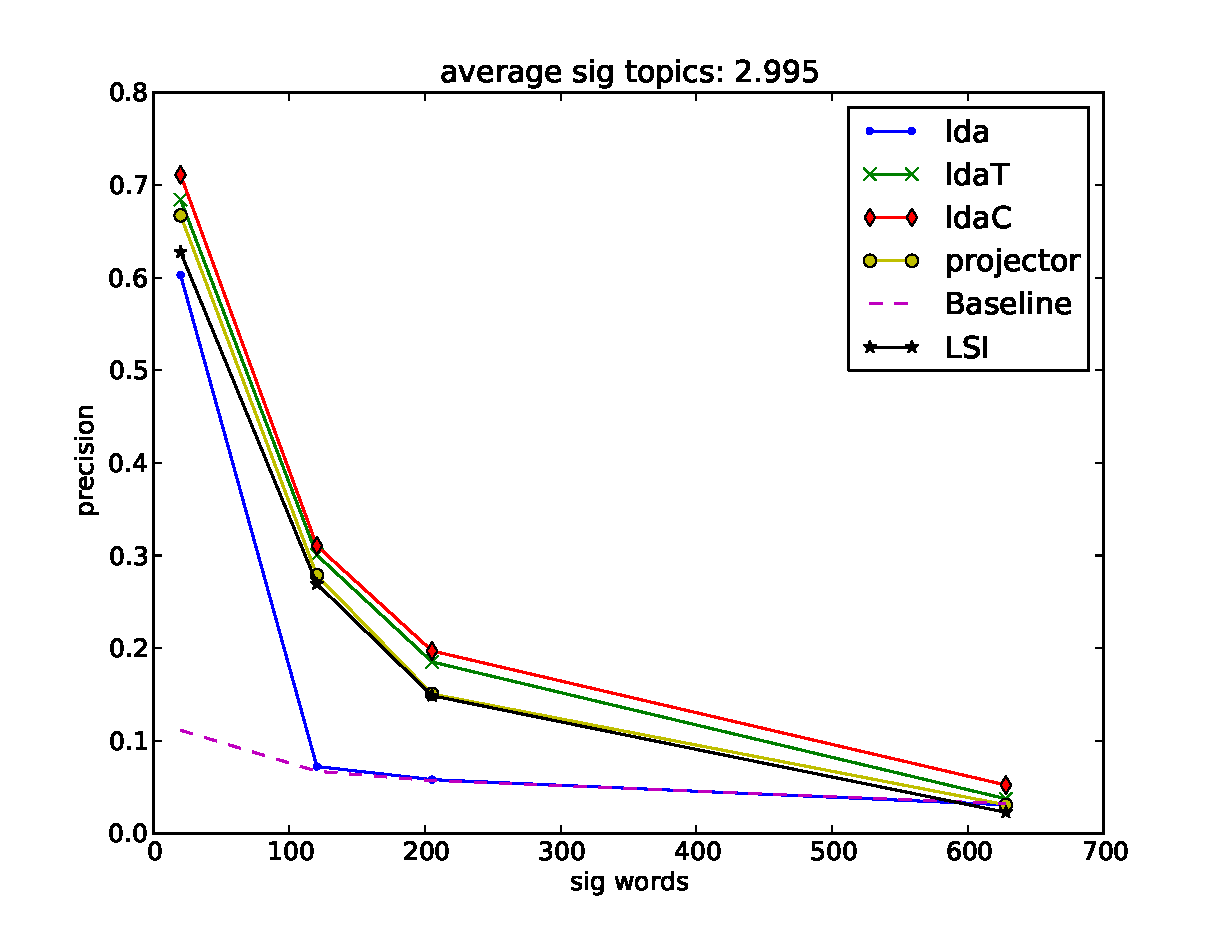
\includegraphics[width=0.4\textwidth]{k20a2995.pdf}
        }\\ 
        \subfigure{
           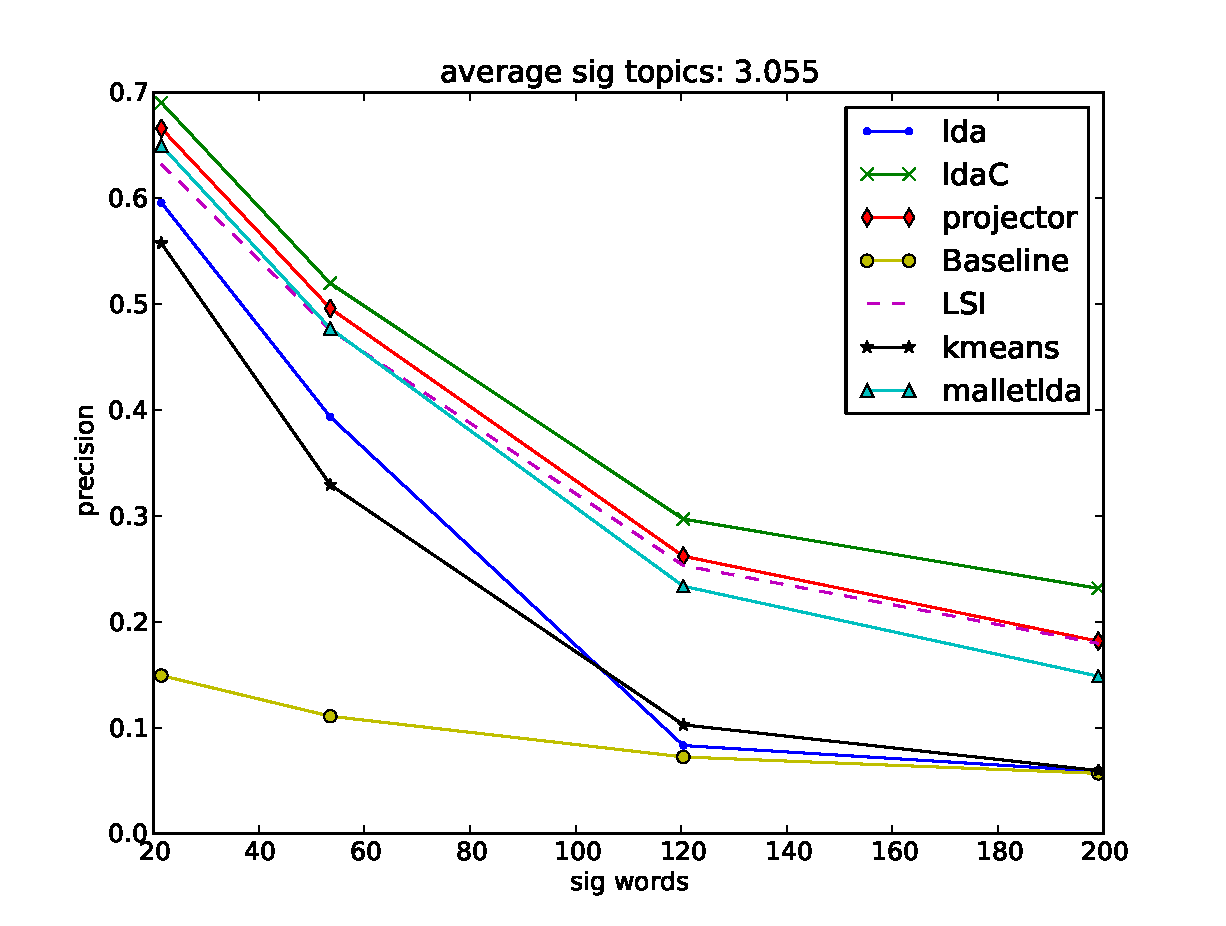
\includegraphics[width=0.4\textwidth]{k15a3.pdf}      
            %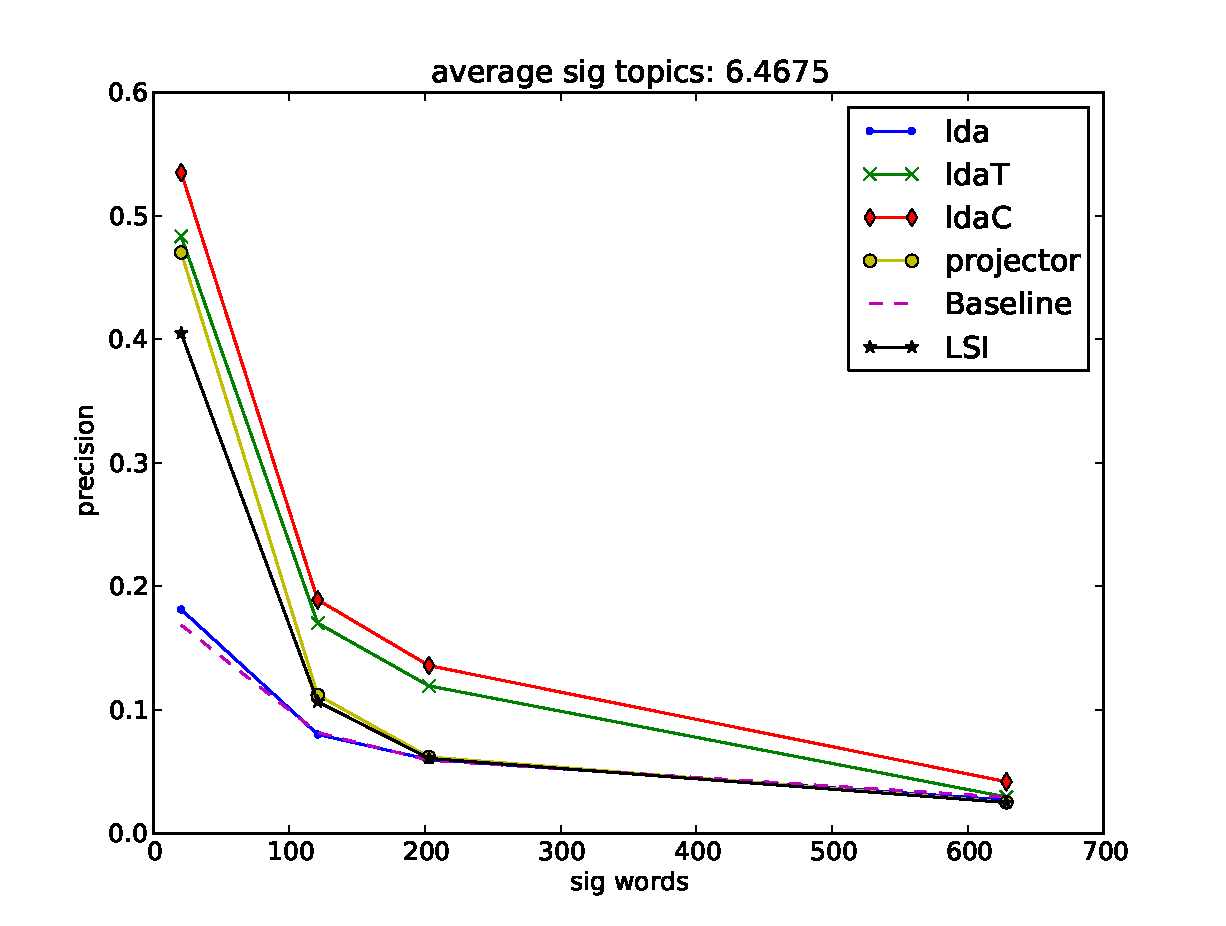
\includegraphics[width=0.4\textwidth]{k20a64675.pdf}
        }
        \subfigure{
           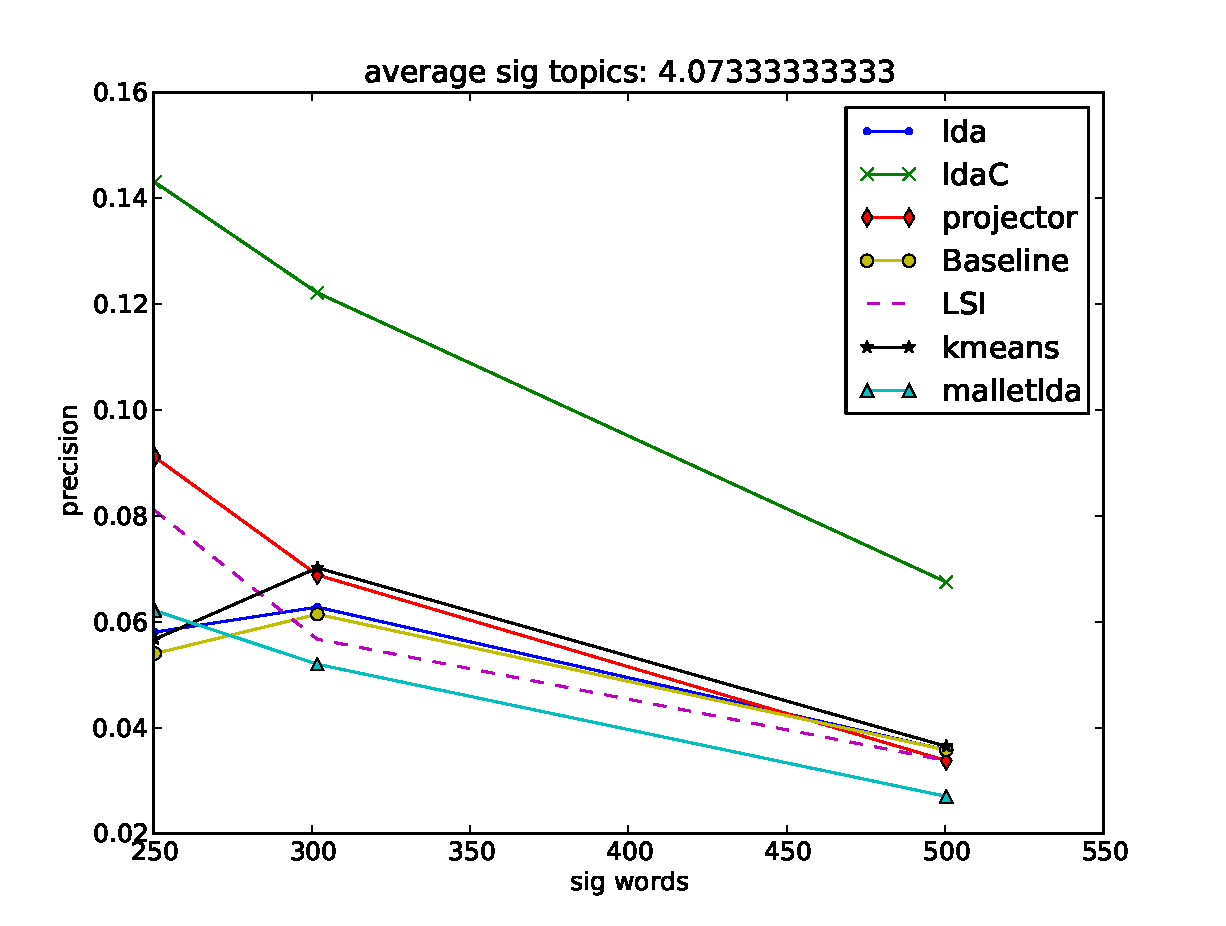
\includegraphics[width=0.4\textwidth]{k15a4.pdf}      
            %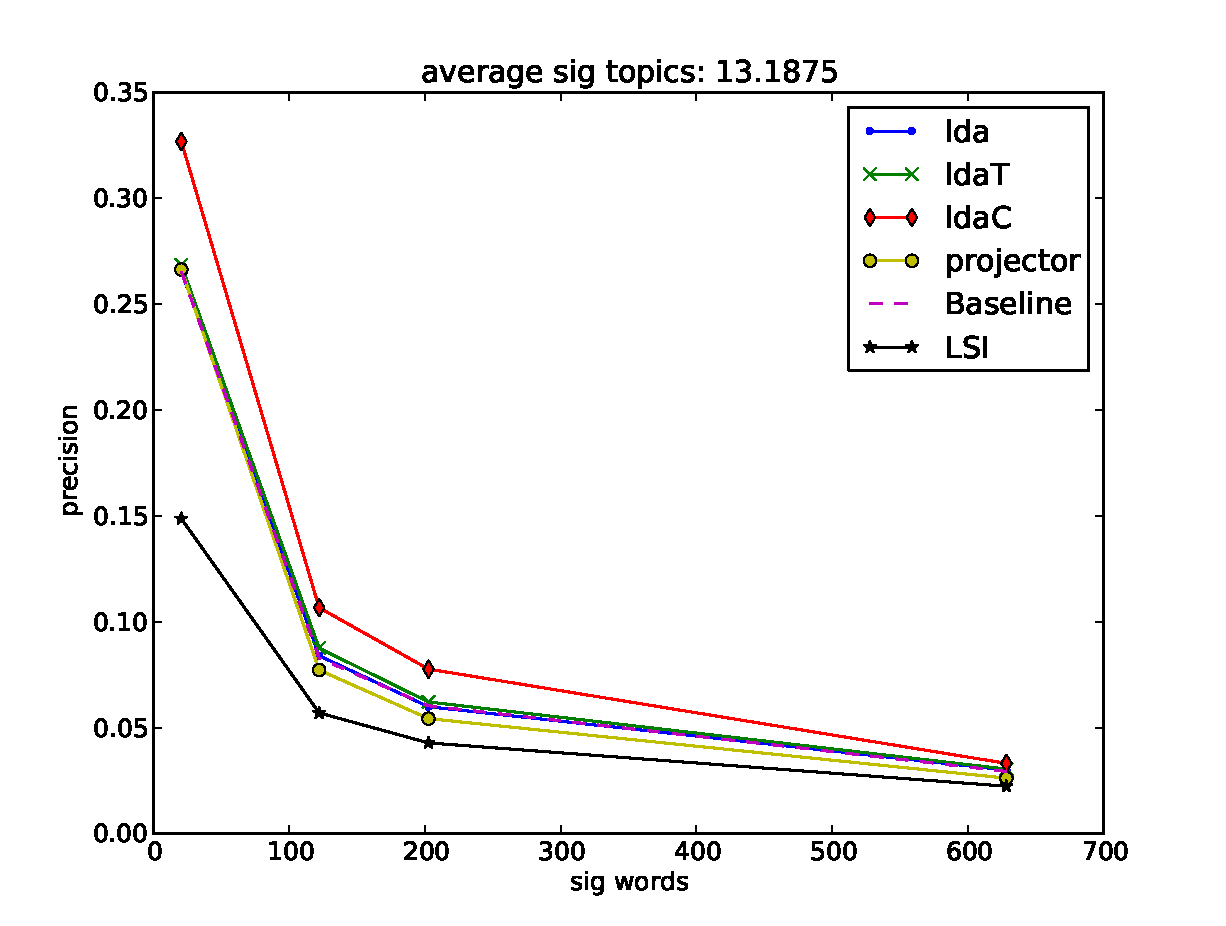
\includegraphics[width=0.4\textwidth]{k20a131875.pdf}
        }

    \end{center}
    \caption{Results of various algorithms on $16$ generated datasets, with $k=20, n=1000,m=1000,l=75$. Each subfigure has a fixed $sig\_topic$, the plots are result of the prediction task versus $sig\_word$}
   \label{fig:predictResult}
\end{figure}

In table~\ref{tab:overall}, we give results for the various algorithms
on the uniform $\alpha$ and $\beta$ datasets.  Here, we see that projector
is competitive with all other algorithms.  In table~\ref{tab:cosine}, we 
give cosine similarity measures for these datasets for mallet lda, k-means,
and projector. 

\begin{table*}
{\tiny
\begin{tabular}{|c|c|c|c|c|c|c|c|c|c|c|}
\hline 
sig\_topics &sig\_words &Baseline &LSI-15 &kmeans-15 &knn-25 &lda-15 &ldaC &ldaT &malletlda-15 &projector-15 \\
 \hline 
5.09  &19.4  &0.21  &0.5  &0.23  &0.46  &0.28  &0.57  &0.54  &0.52  &\textbf{0.54}
  \\
 \hline 
3.03  &199  &0.06  &\textbf{0.18}
  &0.06  &0.15  &0.06  &0.23  &0.23  &0.15  &\textbf{0.18}
  \\
 \hline 
5.01  &53.6  &0.11  &0.3  &0.11  &0.27  &0.12  &0.36  &0.34  &0.31  &\textbf{0.32}
  \\
 \hline 
1.19  &19.73  &0.04  &0.81  &0.81  &0.81  &0.73  &0.84  &0.84  &0.79  &\textbf{0.82}
  \\
 \hline 
7.42  &55  &0.17  &0.21  &0.17  &0.19  &0.17  &0.3  &0.26  &\textbf{0.25}
  &0.23  \\
 \hline 
1.19  &206.13  &0.06  &\textbf{0.32}
  &0.29  &0.31  &0.27  &0.32  &0.32  &0.29  &\textbf{0.32}
  \\
 \hline 
2.46  &53.2  &0.09  &0.53  &0.48  &0.51  &0.49  &0.56  &0.56  &0.52  &\textbf{0.54}
  \\
 \hline 
7.36  &20.6  &0.22  &0.35  &0.22  &0.3  &0.22  &0.48  &0.41  &\textbf{0.41}
  &0.4  \\
 \hline 
3.06  &21.53  &0.15  &0.63  &0.56  &0.59  &0.6  &0.69  &0.66  &0.65  &\textbf{0.67}
  \\
 \hline 
3.07  &120.4  &0.07  &0.25  &0.1  &0.24  &0.08  &0.3  &0.28  &0.23  &\textbf{0.26}
  \\
 \hline 
2.48  &119.53  &0.06  &0.29  &0.18  &0.29  &0.12  &0.32  &0.32  &0.28  &\textbf{0.3}
  \\
 \hline 
2.51  &204.33  &0.06  &0.19  &0.08  &0.15  &0.07  &0.24  &0.23  &0.17  &\textbf{0.22}
  \\
 \hline 
3.06  &53.53  &0.11  &0.48  &0.33  &0.46  &0.39  &0.52  &0.5  &0.48  &\textbf{0.5}
  \\
 \hline 
5.07  &205.67  &0.07  &\textbf{0.09}
  &0.06  &0.06  &0.07  &0.14  &0.13  &0.07  &\textbf{0.09}
  \\
 \hline 
1.2  &51.6  &0.04  &0.68  &0.64  &\textbf{0.69}
  &0.6  &0.71  &0.7  &0.68  &\textbf{0.69}
  \\
 \hline 
5.05  &120.87  &0.08  &0.18  &0.08  &0.14  &0.08  &0.23  &0.21  &0.16  &\textbf{0.2}
  \\
 \hline 
7.37  &116.53  &\textbf{0.1}
  &0.09  &\textbf{0.1}
  &0.09  &\textbf{0.1}
  &0.17  &0.15  &\textbf{0.1}
  &\textbf{0.1}
  \\
 \hline 
2.5  &19.4  &0.12  &0.68  &0.64  &0.66  &0.61  &0.75  &0.73  &0.68  &\textbf{0.72}
  \\
 \hline 
7.39  &208.13  &\textbf{0.08}
  &0.05  &\textbf{0.08}
  &0.05  &\textbf{0.08}
  &0.11  &0.1  &0.07  &0.06  \\
 \hline 
1.18  &118.07  &0.06  &\textbf{0.48}
  &\textbf{0.48}
  &\textbf{0.48}
  &0.42  &0.49  &0.49  &0.47  &\textbf{0.48}
  \\
 \hline 

\end{tabular}

}
\caption{Bold indicates champion non-cheating method for each row.}

\label{tab:overall}
\end{table*}

\begin{table*}

{\tiny
\begin{tabular}{|c|c|c|c|c|c|c|c|c|}
\hline 
sig\_topics &sig\_words &lda-15 &malletlda-15 &projector-15 &~kmeans-cosine &~lda-cosine &~mallet-cosine &~projector-cosine \\
 \hline 
5.09  &19.4  &0.28  &0.52  &\textbf{0.54}
  &0.14  &0.62  &0.98  &0.98  \\
 \hline 
3.03  &199  &0.06  &0.15  &\textbf{0.18}
  &0.45  &0.48  &0.67  &0.88  \\
 \hline 
5.01  &53.6  &0.12  &0.31  &\textbf{0.32}
  &0.23  &0.41  &0.94  &0.95  \\
 \hline 
1.19  &19.73  &0.73  &0.79  &\textbf{0.82}
  &0.15  &0.93  &0.99  &1.0  \\
 \hline 
7.42  &55  &0.17  &\textbf{0.25}
  &0.23  &0.23  &0.37  &0.76  &0.73  \\
 \hline 
1.19  &206.13  &0.27  &0.29  &\textbf{0.32}
  &0.45  &0.81  &0.83  &0.94  \\
 \hline 
2.46  &53.2  &0.49  &0.52  &\textbf{0.54}
  &0.22  &0.84  &0.97  &0.98  \\
 \hline 
7.36  &20.6  &0.22  &\textbf{0.41}
  &0.4  &0.14  &0.39  &0.98  &0.94  \\
 \hline 
3.06  &21.53  &0.6  &0.65  &\textbf{0.67}
  &0.15  &0.91  &0.99  &0.99  \\
 \hline 
3.07  &120.4  &0.08  &0.23  &\textbf{0.26}
  &0.34  &0.49  &0.87  &0.94  \\
 \hline 
2.48  &119.53  &0.12  &0.28  &\textbf{0.3}
  &0.34  &0.59  &0.88  &0.95  \\
 \hline 
2.51  &204.33  &0.07  &0.17  &\textbf{0.22}
  &0.45  &0.49  &0.75  &0.9  \\
 \hline 
3.06  &53.53  &0.39  &0.48  &\textbf{0.5}
  &0.22  &0.75  &0.96  &0.97  \\
 \hline 
5.07  &205.67  &0.07  &0.07  &\textbf{0.09}
  &0.45  &0.46  &0.42  &0.69  \\
 \hline 
1.2  &51.6  &0.6  &0.68  &\textbf{0.69}
  &0.23  &0.84  &0.98  &0.99  \\
 \hline 
5.05  &120.87  &0.08  &0.16  &\textbf{0.2}
  &0.34  &0.41  &0.78  &0.86  \\
 \hline 
7.37  &116.53  &\textbf{0.1}
  &\textbf{0.1}
  &\textbf{0.1}
  &0.33  &0.39  &0.43  &0.58  \\
 \hline 
2.5  &19.4  &0.61  &0.68  &\textbf{0.72}
  &0.14  &0.86  &0.99  &0.99  \\
 \hline 
7.39  &208.13  &\textbf{0.08}
  &0.07  &0.06  &0.46  &0.46  &0.23  &0.41  \\
 \hline 
1.18  &118.07  &0.42  &0.47  &\textbf{0.48}
  &0.33  &0.84  &0.93  &0.97  \\
 \hline 

\end{tabular}

}
\caption{Bold indicates champion results and we use cosine similiarity where matching
to model topics uses maximum weight matching.}
\label{tab:cosine}
\end{table*}

For $\alpha$ chosen so that the topic distribution obeys a power
law, we present results in table~\ref{}. Here, we see that
projector again performs robustly well.  We note that 
the Mallet implementation optimizes over varying values of
$\alpha$. 

\begin{table*}
{\tiny
\begin{tabular}{|c|c|c|c|c|c|c|c|c|c|c|}
\hline 
sig\_topics &sig\_words &Baseline &lda-15 &ldaC &ldaT &malletlda-15 &projector-15 &~lda-cosine &~mallet-cosine &~projector-cosine \\
 \hline 
1.4  &98.73  &{0.12}
  &{0.5}
  &{0.53}
  &{0.52}
  &{0.43}
  &\textbf{0.51}
  &0.95  &0.8  &0.98  \\
 \hline 
3.59  &203  &{0.06}
  &{0.06}
  &{0.18}
  &{0.15}
  &{0.12}
  &\textbf{0.13}
  &0.46  &0.65  &0.87  \\
 \hline 
2.29  &52.93  &{0.13}
  &{0.49}
  &{0.55}
  &{0.54}
  &{0.47}
  &\textbf{0.5}
  &0.91  &0.88  &0.92  \\
 \hline 
3.61  &54.8  &{0.19}
  &{0.19}
  &{0.44}
  &{0.45}
  &{0.35}
  &\textbf{0.43}
  &0.46  &0.79  &0.98  \\
 \hline 
1.69  &100.8  &{0.08}
  &{0.4}
  &{0.45}
  &{0.45}
  &{0.38}
  &\textbf{0.44}
  &0.91  &0.87  &0.97  \\
 \hline 
2.29  &202  &{0.06}
  &{0.07}
  &{0.23}
  &{0.22}
  &{0.19}
  &\textbf{0.21}
  &0.5  &0.73  &0.87  \\
 \hline 
1.38  &204.67  &{0.06}
  &{0.15}
  &{0.34}
  &{0.33}
  &{0.27}
  &\textbf{0.3}
  &0.58  &0.78  &0.95  \\
 \hline 
3.58  &99.53  &{0.16}
  &{0.16}
  &{0.35}
  &{0.35}
  &{0.27}
  &\textbf{0.33}
  &0.44  &0.81  &0.9  \\
 \hline 
1.66  &54.2  &{0.1}
  &{0.58}
  &{0.61}
  &{0.6}
  &{0.47}
  &\textbf{0.58}
  &0.92  &0.89  &0.99  \\
 \hline 
2.27  &97.53  &{0.11}
  &{0.32}
  &{0.37}
  &{0.38}
  &{0.32}
  &\textbf{0.36}
  &0.88  &0.85  &0.97  \\
 \hline 
1.72  &205.2  &{0.06}
  &{0.08}
  &{0.25}
  &{0.23}
  &{0.19}
  &\textbf{0.23}
  &0.52  &0.7  &0.94  \\
 \hline 
1.4  &52.87  &{0.12}
  &{0.61}
  &{0.69}
  &{0.68}
  &{0.6}
  &\textbf{0.64}
  &0.85  &0.91  &0.92  \\
 \hline 

\end{tabular}
}

\caption{Pareto distribution for topics. Bold indicates best non-cheating result
and cosine similarities are included.}
\label{tab:pareto}
\end{table*}

Finally, table~\ref{tab:real} contains results for the word prediction
task on the standard real world datasets we discussed earlier.

\begin{table*}[ht]
{\tiny

\begin{tabular}{|c|c|c|c|c|c|c|c|c|}
\hline 
 &Baseline &LSI-15 &knn-15 &lda-15 &malletlda-15 &projector-15 \\
 \hline 
AP &0.21 &0.3 &0.28 &0.26 &0.26 &0.24 \\
 \hline 
Cacm &0.07 &0.07 &0.12 &0.1 &0.08 &0.1 \\
 \hline 
Cisi &0.13 &0.13 &0.16 &0.15 &0.15 &0.15 \\
 \hline 
Cran &0.18 &0.27 &0.29 &0.25 &0.25 &0.24 \\
 \hline 
Med &0.08 &0.13 &0.13 &0.12 &0.13 &0.13 \\
 \hline 
Nips &0.66 &0.69 &0.77 &0.75 &0.75 &0.68 \\
 \hline 

\end{tabular}

}
\caption{Experiment results on real datasets. We pick the result of the best among a few parameters for each algorithm. We note that increasing the number of topics to 30 does not change the results. }
\label{tab:real}
\end{table*}


Also see table~\ref{tab:real} for prediction results on real datasets.  There we see that
LDA is no longer dominated by LSI and Projector.  Still,  nearest neighbor's performance
dominates.  In the appendix, in table~\ref{tab:aptopics} we show the most popular
words in a sampling of topic vectors recovered by Projector in the AP dataset.

Typically, we saw the topic matching to correlate with prediction performance.
See figure~\ref{fig:size-matters} to see this result. 


\subsection{Runtime}

\begin{figure}
\begin{center}

        \subfigure{
           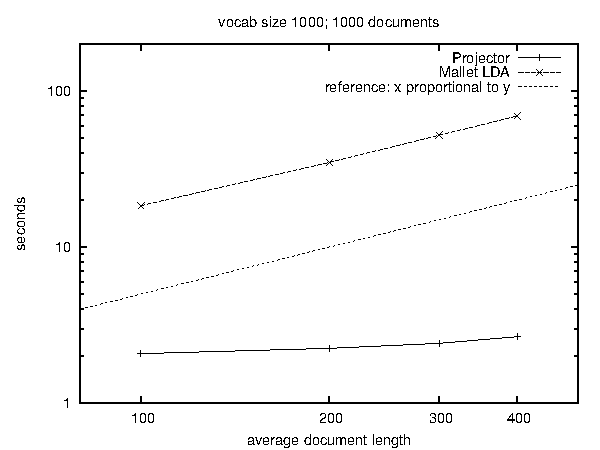
\includegraphics[width=0.4\textwidth]{projector_vs_mallet_doclen.pdf}      
            %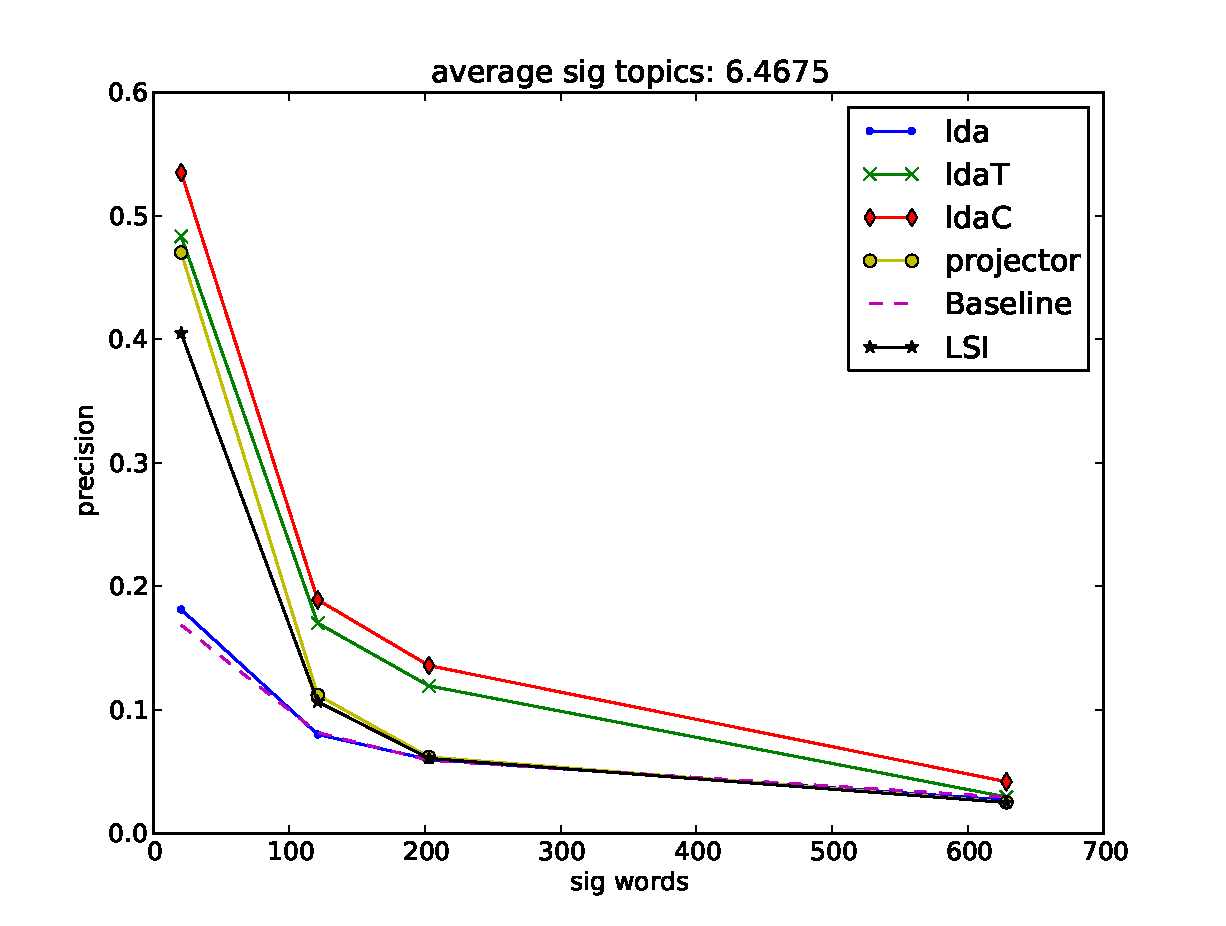
\includegraphics[width=0.4\textwidth]{k20a64675.pdf}
        }
        \subfigure{
           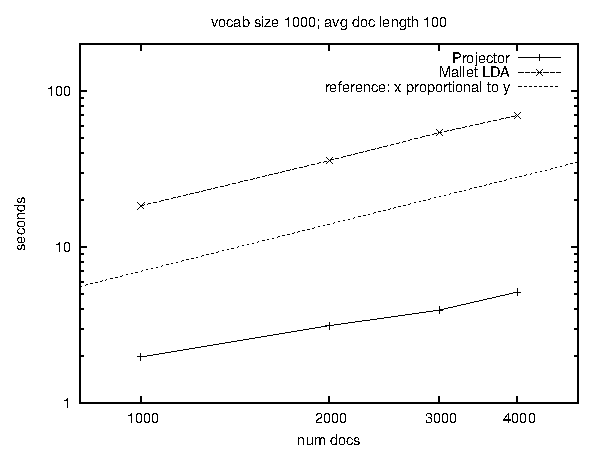
\includegraphics[width=0.4\textwidth]{projector_vs_mallet_ndocs.pdf}      
            %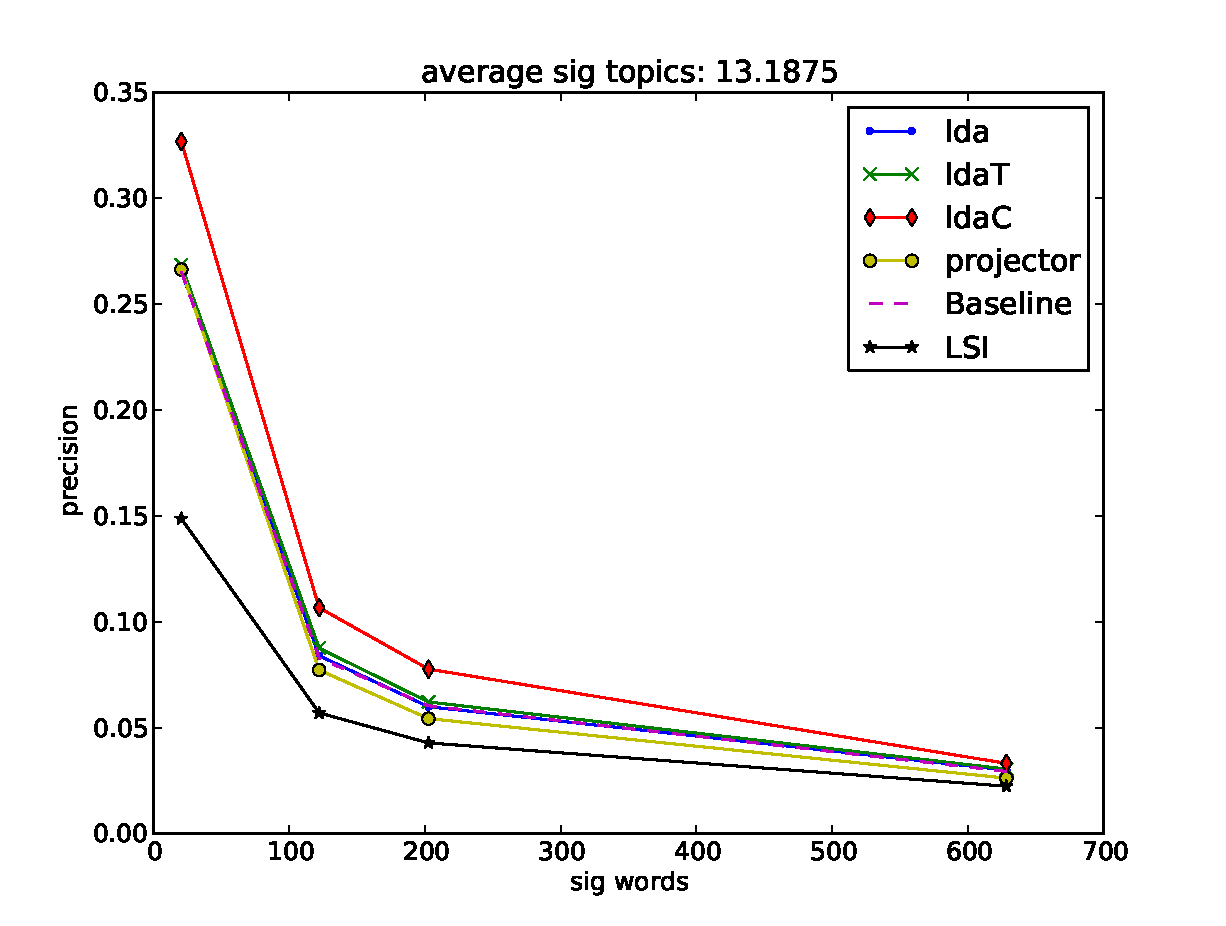
\includegraphics[width=0.4\textwidth]{k20a131875.pdf}
        }
\end{center}
\caption{The runtimes of Mallet's LDA implementation and projector a plotted against
the number of documents and the average document lengths in the figures above. }
\label{fig:time-proj-mallet}
\end{figure}

Figure~\ref{fig:time-proj-mallet}, compares the runtimes of Projector with Mallet
LDA and suggests that Mallet's runtime increases linearly with respect
to average document length and the number of documents.  Projector appears sublinear
in each, which suggests that the our timings are influenced by fixed
startup costs.  Not showen, is Mallet's better scaling with respect
to vocabulary size as Projector uses dense matrices.  Projector's dependence
remains linear in this case. 
